% !TEX program = lualatex
\documentclass[a4paper]{jlreq}
\usepackage[haranoaji]{luatexja-preset}
\usepackage{amsmath}
\usepackage{graphicx}
\usepackage{booktabs}
\usepackage{listings}
\usepackage{pgfplots}
\pgfplotsset{compat=1.17}
\usepackage{xcolor}
\usepackage[hidelinks,pdfusetitle]{hyperref}
\usepackage{url}

% ---- 検証済みパレット（dataviz 基準・印刷面ではダーク段を採用） ----
\definecolor{segcol}{HTML}{C98500}   % 平均同類近傍率（黄・ダーク段）
\definecolor{satcol}{HTML}{008300}   % 満足率（緑）
\definecolor{grpA}{HTML}{2A78D6}     % グループA（青）
\definecolor{grpB}{HTML}{1BAF7A}     % グループB（アクア）
\definecolor{codebg}{HTML}{F5F4F0}

\lstset{
  basicstyle=\ttfamily\small,
  backgroundcolor=\color{codebg},
  frame=single, framerule=0.2pt, rulecolor=\color{black!25},
  breaklines=true, columns=fullflexible, keepspaces=true,
  showstringspaces=false,
  xleftmargin=1em, xrightmargin=1em,
  aboveskip=1em, belowskip=1em
}
\renewcommand{\lstlistingname}{リスト}

\title{{\Large アーティファクトを用いたシミュレーションモデルの作成}\\
  {\small --- Claude Code によるブラウザ内シミュレーションの技術チュートリアル ---}}
\author{河合勝彦\thanks{名古屋市立大学大学院経済学研究科　\texttt{kkawai@econ.nagoya-cu.ac.jp}}}
\date{2026年7月12日}

\begin{document}
\maketitle

\begin{abstract}
本稿は，コーディングエージェント Claude Code（Anthropic 社）が備える「アーティファクト」機能（対話から生成した Web ページを固定 URL で公開する仕組み）を用いて，ブラウザ内で完結するインタラクティブ・シミュレーションを構築するための技術チュートリアルである．まず Claude Code とアーティファクトの機能・発動条件・技術的制約を整理し，設計を支援する二つのスキル（Claude Code に読み込ませる指針書 \texttt{artifact-design}・\texttt{dataviz}）の役割を説明する．次に，制作過程の実例として，（1）連続時間の状態遷移と採点関数をもつ遊戯的シミュレータ「炭火職人」（うなぎ蒲焼きシミュレータ），（2）標準仕様のシェリング分居モデルのライブ実行環境，の二つを取り上げ，設計判断・実装・検証の全過程を示す．さらにシェリングモデルについては，アーティファクトと同一アルゴリズムの再現実行により得た分析結果（許容閾値 $\tau=0.3$ における分居の創発，$\tau$ と分居度の非線形関係，収束時間の急増）を報告する．社会科学分野の学生・研究者を読者に想定し，情報技術の専門用語と略語には本文中で解説を付す．

\par\bigskip\noindent
\textbf{キーワード：}エージェント・ベース・モデル（ABM），シェリング分居モデル，コーディングエージェント，Claude Code，アーティファクト，再現性，データ可視化
\end{abstract}

\tableofcontents

\section{はじめに}

エージェント・ベース・モデル（agent-based model; ABM），すなわち多数の主体（エージェント）に単純な行動規則を与え，その相互作用から生じるマクロな帰結を計算機上で観察する手法の研究・教育において，「モデルに触れられる」デモンストレーションの価値は大きい．パラメータを動かした瞬間にマクロな帰結が変わる体験は，数式やソースコードの静的な提示では代替できない．しかし従来，この種のデモを配布するには，ABM 用の統合環境である NetLogo の導入，Web サーバの運用，あるいは JavaScript（Web ブラウザ上で動作するプログラミング言語）のフレームワーク（開発の土台となるライブラリ群）の学習といった準備コストが必要であった．

Claude Code（Anthropic 社が提供するコーディングエージェント，第\ref{sec:artifact}節で詳述）のアーティファクト（Artifact）機能は，この準備コストを大幅に引き下げる．対話的に仕様を伝えるだけで，自己完結した HTML（HyperText Markup Language：Web ページを記述する言語）のアプリケーションが \texttt{claude.ai} 上の固定 URL（Uniform Resource Locator：Web 上の所在を示すアドレス）に公開され，閲覧を許可された相手はブラウザだけで実行できる（共有できる範囲は契約プランに依存する；第\ref{sec:artifact}節）．本稿では，この機能を用いたシミュレーション構築の技術的要点を，実際の制作過程に即して解説する．

なお本稿は，社会科学分野の学生・研究者を主な読者に想定し，Web 技術やプログラミングの予備知識を前提としない．情報技術の専門用語は初出時に本文中で短く解説し，略語（アクロニム）には初出時に正式名称を併記する．

本稿の構成は次のとおりである．第\ref{sec:artifact}節で Claude Code とアーティファクトの機能・制約を整理する．第\ref{sec:kabayaki}節では第一の事例として，連続時間の状態遷移をもつ遊戯的シミュレータの設計と実装を示す．第\ref{sec:schelling}節では第二の事例として，シェリング分居モデルの標準仕様による実装と，その分析結果を報告する．第\ref{sec:discussion}節で教育・研究上の含意と限界を論じる．

\section{Claude Code とアーティファクト}\label{sec:artifact}

\subsection{Claude Code とは}

アーティファクトの説明に先立ち，その土台である Claude Code 自体について述べる．Claude Code は Anthropic 社が提供する\textbf{コーディングエージェント}（coding agent）である\cite{anthropic-claudecode}．ここでの「エージェント」は本稿の主題である ABM のエージェントとは別義であり，大規模言語モデル（large language model; LLM）\footnote{対話型の人工知能（AI; artificial intelligence）の中核にある，大量のテキストから学習した言語処理モデル．}が，ファイルの読み書き・シェルコマンド（コンピュータを文字入力で操作する命令）の実行・Web 検索といった\textbf{ツール}を自律的に呼び出しながら，与えられた目標を達成するまで作業を続けるソフトウェアを指す．

従来の対話型 AI（チャットボット）との本質的な違いは，応答が「テキストの生成」で完結しない点にある．チャットボットはコードを提示できても，それを実行するのは利用者の仕事である．これに対し Claude Code は，利用者が自然言語で目標を伝えると，作業計画を立て，コードを書き，それを実際に実行して結果を観察し，エラーや仕様とのずれがあれば自ら修正する—という「編集・実行・検証」のサイクルを，逐次の指示を待たずに繰り返す．本稿の制作過程でも，HTML/JavaScript の実装だけでなく，配色の検証スクリプト（ひとまとまりの処理を自動実行する小さなプログラム）の実行（第\ref{sec:palette}節），Node.js（ブラウザの外で JavaScript を実行する環境）によるパラメータスイープ\footnote{パラメータ値を系統的に変えながらシミュレーションを一括実行する実験．}（第\ref{sec:analysis}節），そしてアーティファクトとしての公開までが，同一エージェントの一連のツール呼び出しとして行われた．

Claude Code は端末のコマンドラインツール（文字入力で対話する画面）のほか，デスクトップアプリ，Web ブラウザ（\texttt{claude.ai/code}），IDE（integrated development environment；統合開発環境）の拡張機能として利用できる．本稿で扱うアーティファクトは，このエージェントが備えるツールの一つ（生成した HTML を \texttt{claude.ai} 上に公開する機能）であり，後述するスキルは，エージェントが特定の種類の作業に着手する前に読み込む指針書である．すなわち本稿のワークフロー（対話による仕様確定，設計，実装，検証，公開，分析）は，すべて単一のコーディングエージェントとの対話の中で完結している．

\subsection{アーティファクトとは}

アーティファクトは，Claude が生成した HTML または Markdown（見出しや箇条書きを記号で簡便に表す文書記法）のファイルを \texttt{claude.ai} 上の Web ページとして表示（レンダリング）し，固定 URL で配信する仕組みである\cite{anthropic-artifacts}．重要な性質は以下のとおり．

\begin{itemize}
  \item \textbf{既定で非公開}\quad 公開直後は作成者本人のみが閲覧できる．Team・Enterprise プランでは，ページの共有メニューから組織内の相手に閲覧を許可できる（組織外への Web 公開はできない）．個人プラン（Pro・Max）では本人のみの閲覧となるため，第三者に渡すには自己完結した HTML ファイル自体を配布する（受け取った側はブラウザで開くだけで実行できる）\footnote{なお，チャット UI（\texttt{claude.ai} の会話画面）で作成されるアーティファクトは，本稿で扱う Claude Code のものとは別の仕組みで，共有の規則も異なる．チャット UI 版は，個人プラン（Free・Pro・Max）では「公開（Publish）」操作により誰でも閲覧できる公開リンクを発行できる（Team・Enterprise では組織内共有のみ）\cite{anthropic-publish}．一方，Claude Code 版には一般公開の手段がない．組織外へ配布するには，HTML ファイルの直接配布のほか，GitHub Pages 等の静的ホスティングによる公開が使える（第\ref{sec:ghpages}節）．}．
  \item \textbf{固定 URL と更新}\quad 同一ファイルパスから再公開すると同じ URL の内容が更新される．バージョンにはラベルを付与でき，履歴をたどれる．
  \item \textbf{静的配信}\quad サーバ側（サーバサイド）の計算資源は付かない．動的な挙動はすべてクライアント側（閲覧者のブラウザ）の JavaScript が担う．
\end{itemize}

\subsection{発動条件と基本ワークフロー}

アーティファクトは自動的に作られるものではなく，(a) 利用者が明示的に依頼した場合（「デモを作って」「Web ページにして」），(b) 端末のテキスト出力よりページとして見せる方が明らかに適切だと Claude が判断した場合に，ツール呼び出しとして発動する．シミュレーション構築の典型的なワークフローは次のとおりである．

\begin{enumerate}
  \item \textbf{仕様の対話的確定}\quad モデルの状態変数・更新規則・操作したいパラメータ・観察したい指標を自然言語で伝える．「標準的な仕様で」という指示も有効に機能する（第\ref{sec:schelling}節の事例）．
  \item \textbf{デザインプランの提示}\quad Claude が配色・タイポグラフィ（書体の選択と文字の組み方）・レイアウトの計画を明示する（\texttt{artifact-design} スキル，次項）．
  \item \textbf{実装}\quad 単一の HTML ファイルとして CSS（Cascading Style Sheets：ページの見た目を記述する言語）と JavaScript を含めて書き下ろす．
  \item \textbf{公開}\quad Artifact ツールで URL が発行される．修正依頼は同じ URL への再公開として反映される．
\end{enumerate}

なお，本稿に掲載する実行画面（図\ref{fig:kabayaki-ui}〜図\ref{fig:schelling-live}）はすべて，公開済みアーティファクトと同一の HTML をブラウザで実行して撮影したものである．

\subsection{設計を支援する二つのスキル}

制作品質は二つのスキル（Claude Code に読み込ませる指針書）に支えられている．

\paragraph{artifact-design}
ページ制作前に必ず読み込む設計指針である．依頼を「実用的な扱い」と「エディトリアルな扱い」に読み分け\footnote{前者は文書・計画書など情報伝達が主目的のもの．後者は雑誌の誌面のように固有の世界観を打ち出す扱いで，ランディングページ（製品などを紹介する 1 枚構成の Web ページ）・ゲーム・共有されるツールなどが該当する．}，後者では定型的な出力（いわゆる AI 的デザイン）を避けて題材固有の視覚言語を構築することを要求する．コードを書く前に，配色（4〜6 色の名前付きパレット）・書体（役割別に 2 種以上）・レイアウト構想からなる「デザインプラン」を明示する手続きが定められている．

\paragraph{dataviz}
チャートを一つでも含む場合に読み込む作図規範である．特徴は「色は計算で検証する」という原則にあり，付属の検証スクリプトが (1) 明度帯域，(2) 彩度下限，(3) 色覚多様性（color vision deficiency; CVD）の下での色の分離度\footnote{CVD は色の見え方が多数派と異なる特性．分離度は，Machado ら（2009）の手法で色覚特性をシミュレートしたうえで，色差指標 $\Delta E$（色同士の見た目の隔たり）として算出する．}，(4) 背景とのコントラスト比（図や文字と背景の明るさの比）を機械的に判定する．本稿の事例でも全系列色をこの検証に通した（第\ref{sec:palette}節）．このほか，二重軸（左右で目盛りが異なる 2 本の縦軸）の禁止，2 系列以上での凡例必置，データ色を文字に使わない，等の規則が定められている．

\subsection{技術的制約}\label{sec:constraints}

シミュレーション設計上，特に重要な制約は三つある．

\begin{description}
  \item[完全な自己完結（CSP）] 厳格な CSP（Content Security Policy）\footnote{ページが外部のサーバと通信することを制限する，ブラウザの安全機構．}により，外部ホストへの一切の通信が遮断される．遮断対象には，CDN（content delivery network）\footnote{ライブラリやフォントなどの汎用ファイルを配信する外部のサーバ網．}から読み込むライブラリ，Web フォント，外部画像，および \texttt{fetch}・XHR（XMLHttpRequest）・WebSocket といったプログラムによる通信が含まれる．したがって D3.js 等の可視化ライブラリを使う場合はインライン化（コードを HTML 内へ直接埋め込むこと）が必要であり，実務上は素の JavaScript と Canvas API\footnote{API（application programming interface）は，プログラムから機能を呼び出す窓口の総称．Canvas はブラウザ標準の描画機能．}で書くのが素直である．データも HTML 内に埋め込む．
  \item[サーバサイド計算の不在] Python（統計・データ分析で広く使われるプログラミング言語）の実行環境や NetLogo エンジンへの接続はできない．モデルは JavaScript へ移植してブラウザ内で実行するか，重い計算は事前に別環境で実行し，結果（軌道データ）を埋め込んだ「再生ビューア」として設計する．規模の目安として，Canvas 2D 描画で数千〜1万エージェント，WebGL（Web Graphics Library：画像処理チップを直接使う高速描画方式）の点描画に切り替えれば数十万エージェントまで実用的である．
  \item[状態の非永続性] ページを再読み込みすると初期状態に戻る．再現性はシード付き乱数\footnote{種（シード）と呼ぶ初期値が同じなら，常に同じ数列を生む擬似乱数．}で担保する（第\ref{sec:schelling}節）．
\end{description}

このほか，閲覧者の OS（operating system；基本ソフト）のテーマ設定（明るい配色のライト／暗い配色のダーク）に応じてページが表示されるため，配色は CSS カスタムプロパティ\footnote{色などの値に名前を付けて一元管理する CSS の仕組み．デザイントークンとも呼ばれる．}として定義し，両テーマ分を用意するのが原則である（リスト\ref{lst:tokens}）．

\begin{lstlisting}[caption={テーマ・トークンの定義パターン（抜粋）},label={lst:tokens}]
:root{ --surface:#fcfcfb; --ink:#0b0b0b; --sA:#2a78d6; }
@media (prefers-color-scheme: dark){
  :root{ --surface:#1a1a19; --ink:#ffffff; --sA:#3987e5; }
}
:root[data-theme="light"]{ /* viewer toggle overrides */ }
:root[data-theme="dark"]{  /* both directions          */ }
\end{lstlisting}

Canvas 描画はこのトークンの現在値を \texttt{getComputedStyle} で読み取って着色し，テーマの切替（OS 設定の変化や閲覧者によるページ内の切替ボタンの操作）を監視して再描画する．

\section{事例1：蒲焼きシミュレータ「炭火職人」}\label{sec:kabayaki}

\subsection{題材とデザインプラン}

第一の事例は，浜名湖うなぎの蒲焼きを炭火で焼き上げる遊戯的シミュレータである\footnote{公開 URL: \url{https://claude.ai/code/artifact/100b5bc4-c60e-42cd-9e19-f9277dbb6685}（既定で非公開）．}．「インタラクティブなデモ」という短い依頼から出発し，リポジトリの既存コンテンツ（浜名湖うなぎ紹介サイト）に題材を接地させた．遊戯的な題材だが，内部は連続時間の状態遷移モデルであり，ABM 的なシミュレータ構築の基本要素（状態変数・更新則・操作・評価関数・可視化）をすべて含む．

デザインプランでは「夜の焼き場」という単一の視覚世界に振り切ることを選択し，例外規定（意図的な単一テーマ）を適用して墨色の地に熾火色をアクセントとするダークテーマのみで構成した．タイポグラフィは見出し・引用に明朝，UI（user interface）\footnote{ボタンやメーターなど，利用者が操作・確認する画面要素の総称．}にゴシック，格言「串打ち三年，裂き八年，焼き一生」を縦書き（\texttt{writing-mode: vertical-rl}）で配置している．

図\ref{fig:kabayaki-ui}に開始直後の画面を示す．中央の焼き台は Canvas 2D による動的描画で，熾火の明滅・煙・炎がリアルタイムに変化する．その下の HUD（Head-Up Display）\footnote{ゲーム画面に常時表示される状態情報表示．前を向いたまま計器情報を読める航空機の投影装置に由来する．}には炭の火力，両面（身側・皮側）の焼き加減，タレ回数のメーターが並び，いま炭側（下向き）を向いている面をバッジ（状態を示す小さなラベル表示）で示す．操作は「団扇であおぐ」「裏返す」「タレにくぐらせる」「仕上げる」の 4 ボタンに集約されている．この時点で「タレにくぐらせる」が無効化されているのは，次項で述べるフェーズゲート（所定の条件を満たすまで次の操作を解禁しない仕組み）による．メーター上部のヒント行は，内部状態に応じた助言（優先度付きの規則群として実装）を表示し，チュートリアルなしでも遊べる誘導の役割を担う．

\begin{figure}[tbp]
\centering
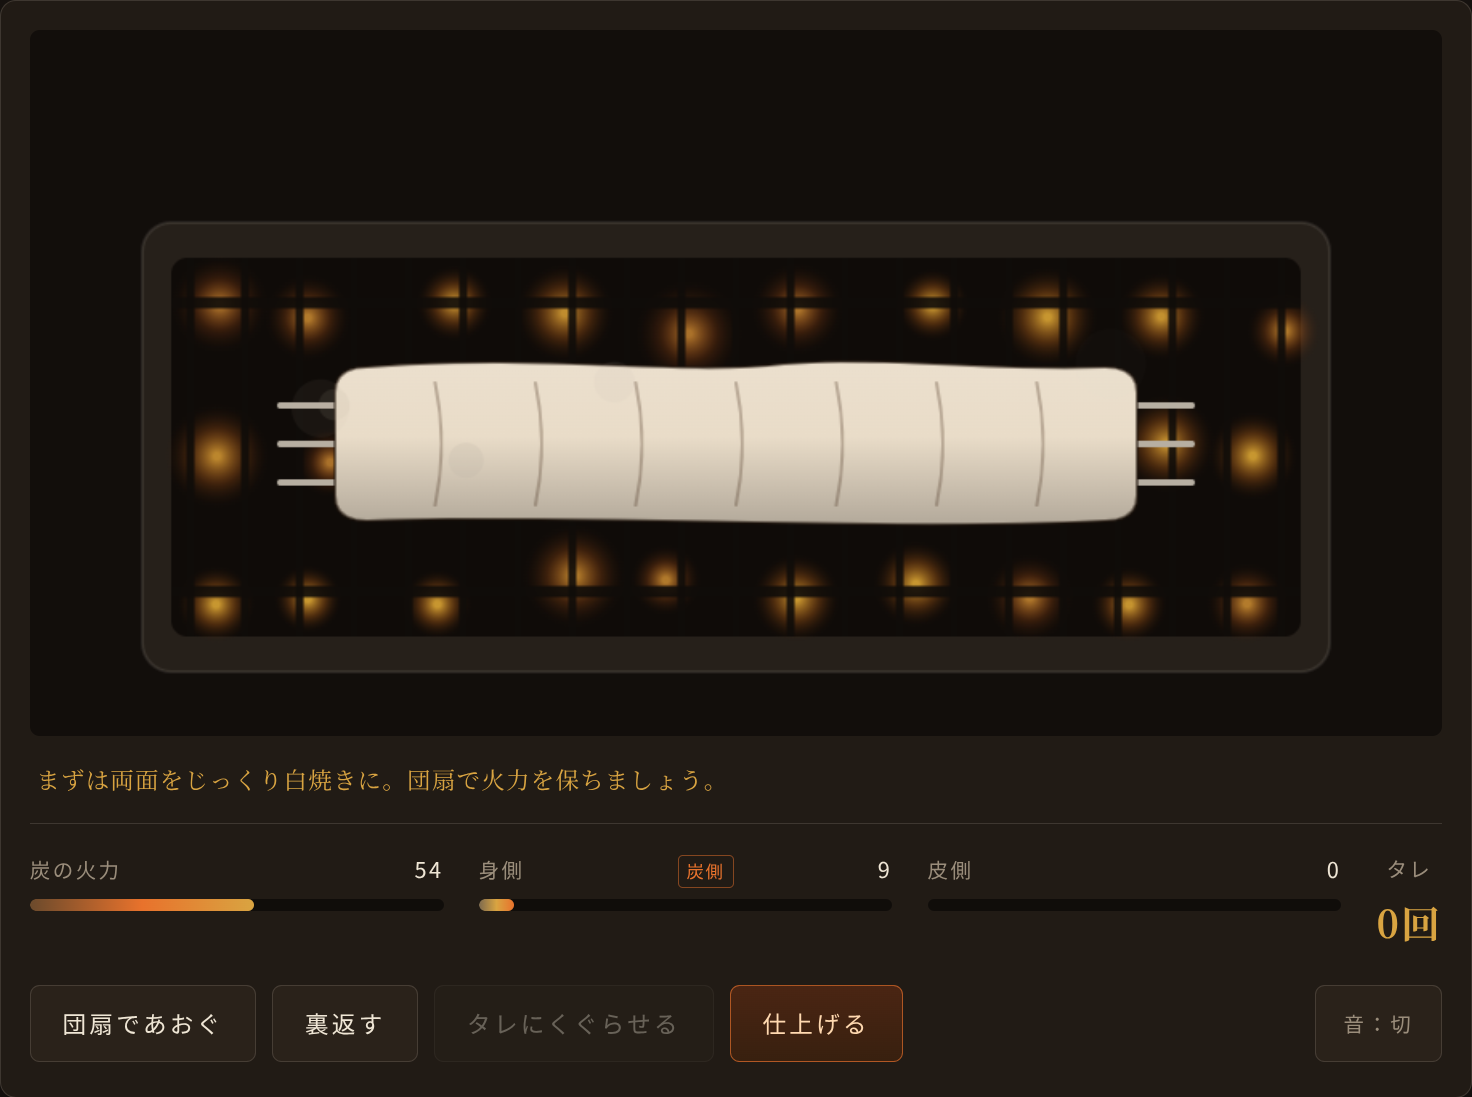
\includegraphics[width=0.92\linewidth]{figures/kabayaki-initial.png}
\caption{「炭火職人」開始直後の画面．Canvas 描画の焼き台（熾火・網・串打ちした鰻），HUD（炭の火力・両面の焼き加減・タレ回数），4 つの操作ボタン．白焼きが完了するまで「タレにくぐらせる」は無効化されている．}
\label{fig:kabayaki-ui}
\end{figure}

\subsection{モデル：状態変数と更新則}

プレイヤーが操作するのは「団扇であおぐ」「裏返す」「タレにくぐらせる」「仕上げる」の 4 ボタンのみである．内部状態は火力 $h(t) \in [30,100]$，両面の焼き加減 $D_i(t)$（$i \in \{\text{身側},\text{皮側}\}$），焦げ量 $C_i(t)$，タレ回数 $n$，タレ湿潤の残り時間 $w(t)$ である．更新則は毎フレーム（画面更新の 1 コマごと，毎秒約 60 回；時間刻み $\Delta t$）：

\begin{align}
  \frac{dh}{dt} &= \kappa\,(h^{*} - h), & \kappa &= 0.055,\ h^{*} = 46
  \label{eq:heat}\\
  \frac{dD_{d}}{dt} &= \rho(h)\,\beta(w), &
  \rho(h) &= 13\cdot\frac{h-30}{70},\quad
  \beta(w) = \begin{cases}1.25 & (w>0)\\ 1 & (w \le 0)\end{cases}
  \label{eq:cook}\\
  \frac{dC_{d}}{dt} &= 0.85\,\rho(h)\,\mathbf{1}[D_{d} > 100]
  \label{eq:char}
\end{align}

ここで $d$ は炭側（下）を向いている面を表し，「裏返す」操作が $d$ を切り替える．「団扇」は $h \leftarrow \min(100,\,h+16)$ の離散ジャンプである．式\eqref{eq:heat}の時定数（平衡値との差が約 63\%縮むまでの時間）は約 18 秒であり，放置すれば火力は熾火の平衡値 46 に緩和する．プレイヤーは団扇による離散介入で $h$ を管理し，式\eqref{eq:cook}の焼成速度を制御する—これが本作の中核的なトレードオフ（高火力は速いが式\eqref{eq:char}の焦げリスクを増す）を生む．

タレは両面が白焼き基準（$D_i \ge 50$）に達するまで解禁されないフェーズゲートをもち，「仕上げる」で評価関数
\begin{equation}
  S = 100 - \sum_i b(D_i) - 1.2\sum_i C_i - P(n),\qquad
  b(D) = 0.9\,(70-D)_{+} + 0.8\,(D-95)_{+}
\end{equation}
が計算される（$(x)_{+} = \max(x,0)$）．$P(n)$ はタレ回数のペナルティで $n=2,3$ を最適とする．焼き加減の理想帯 $[70,95]$・焦げ係数・タレ最適回数という 3 つの評価軸が互いに緊張関係にあるため，単調な攻略法が存在しない．

\subsection{実装のポイント}

描画は Canvas 2D で行い，\texttt{requestAnimationFrame}\footnote{ブラウザの画面更新周期（毎秒約 60 回）に同期して処理を繰り返す仕組み．}のループ内で状態更新と描画を分離した．熾火の明滅は決定的擬似乱数と正弦波の合成，煙・炎は簡易パーティクル系\footnote{多数の微小な粒を生成・移動させて，煙や炎などの流動的な現象を表す描画技法．}（生成率を $h$ と $w$ に比例させる）で表現している．タレが炭に落ちて炎が上がる演出は，実際の蒲焼きの物理に対応した「モデルに正直な」エフェクトである．アクセシビリティ（心身の特性や利用環境によらず使えるようにする配慮）として，OS の「視覚効果を減らす」設定（\texttt{prefers-reduced-motion}）の利用時はパーティクルを停止し，効果音\footnote{WebAudio（ブラウザ標準の音声処理機能）を用い，白色雑音（あらゆる高さの成分を均等に含む雑音）を帯域フィルタに通して合成した．音量は火力 $h$ に追従する．}は既定オフのトグル（オン・オフ切替）とした．

図\ref{fig:kabayaki-tare}は，両面の白焼きを終えてタレに 1 度くぐらせた直後の局面である．鰻は飴色の照りをまとい（タレ回数と湿潤状態に応じてグレーズと光沢の描画を重ねている），ヒント行は「タレが炭に落ちて炎が上がる」ことを告げる．HUD からは両面の焼き加減がともに 70 に達し，皮側が炭側を向いていることが読み取れる．

\begin{figure}[tbp]
\centering
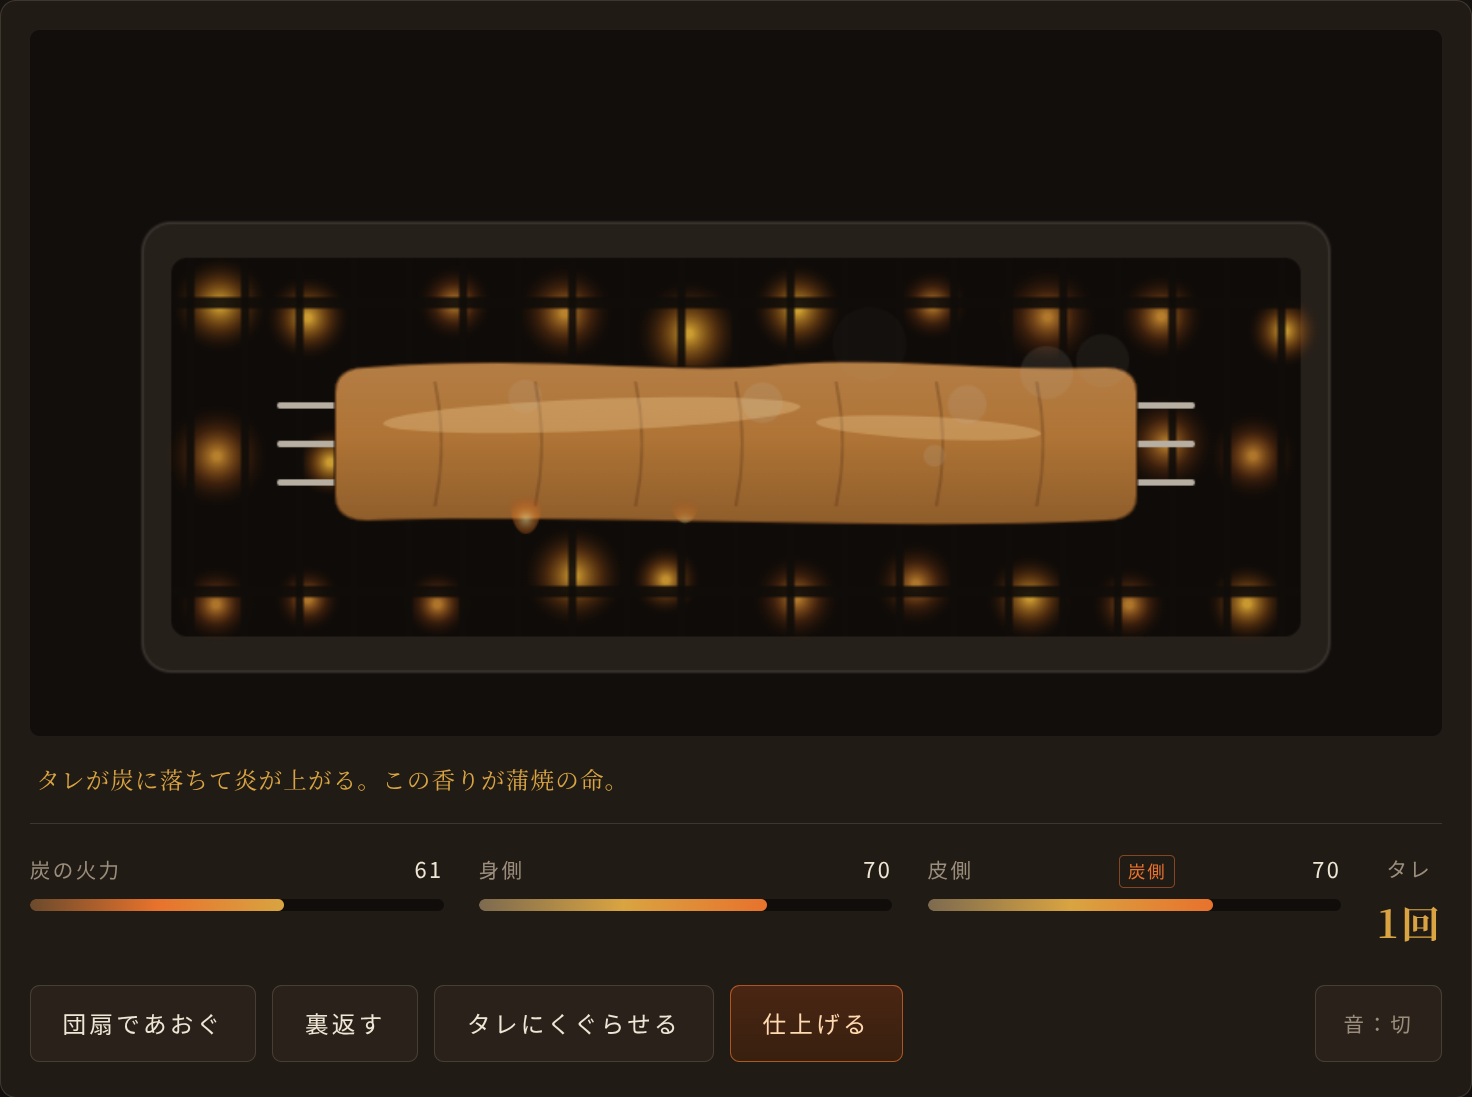
\includegraphics[width=0.92\linewidth]{figures/kabayaki-tare.png}
\caption{タレ焼きの局面．両面の白焼き（各 70）を終えてタレを 1 度まとった状態．タレの湿潤中（$w>0$）は焼成が 1.25 倍に加速し，炭に落ちたタレが炎を上げる．HUD の「炭側」バッジは皮側が下を向いていることを示す．}
\label{fig:kabayaki-tare}
\end{figure}

\subsection{評価画面}

「仕上げる」を押すと式\eqref{eq:heat}--\eqref{eq:char}の履歴に基づいて評価関数が計算され，朱漆の重箱に盛られた結果画面が表示される（図\ref{fig:kabayaki-result}）．図の例は，身側 82・皮側 82・タレ 2 回・焦げ僅少で評点 100（番付「匠」）を得た一枚である．結果画面には評価の内訳（両面の焼き加減・タレ回数・焦げ量）が明示されるため，プレイヤーは何が加点・減点の要因だったかを事後的に確認し，次の一枚に反映できる．焼き加減の理想帯 $[70,95]$ はタレの湿潤ブースト（1.25 倍）を考慮すると意外に狭く，仕上げの数秒を誤るだけで焦げが急速に蓄積する—この時間的な緊張感が本作の遊戯性の中心である．

\begin{figure}[tbp]
\centering
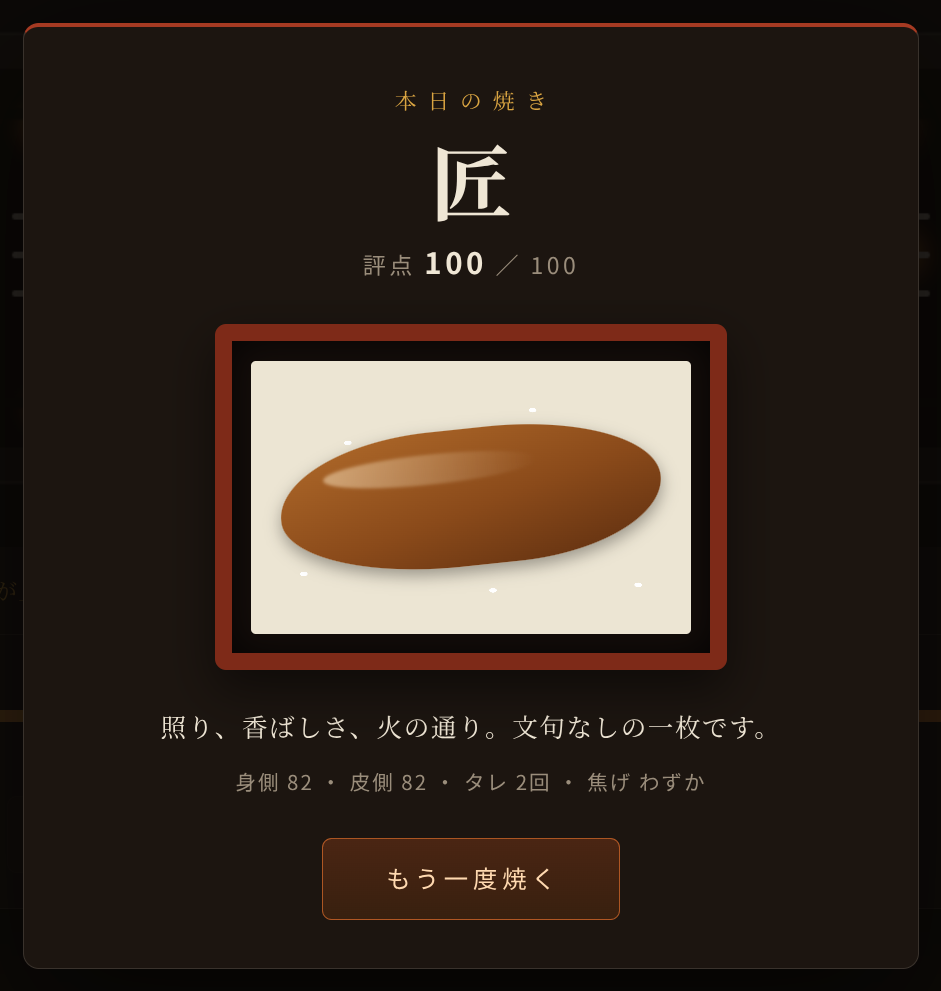
\includegraphics[width=0.5\linewidth]{figures/kabayaki-result.png}
\caption{評価画面．身側 82・皮側 82・タレ 2 回・焦げ僅少で評点 100・番付「匠」．重箱と鰻は CSS のみで描画され，焼き上がり（生焼け・良好・焦げ）に応じて色が変わる．}
\label{fig:kabayaki-result}
\end{figure}

\section{事例2：シェリング分居モデル}\label{sec:schelling}

\subsection{モデル仕様}

第二の事例は Schelling (1971) の分居モデルの標準仕様によるライブ実行環境である\footnote{公開 URL: \url{https://claude.ai/code/artifact/9ac47541-7715-48f8-9513-39ef5e4c9772}（既定で非公開）．}．依頼は「モデル仕様は標準的なもので」であり，実装した仕様は次のとおり．

\begin{itemize}
  \item $L \times L$ 正方格子．境界は周期境界（トーラス：上端と下端・左端と右端をつないだドーナツ状の構造）．近傍はムーア近傍（上下左右と斜めを合わせた 8 マス）．
  \item 2 グループのエージェント．全セルから空き地率 $v$ 分を除き，指定比率で配分してランダム配置．
  \item 満足条件：占有近傍セルに占める同類の割合が許容閾値 $\tau$ 以上（占有近傍が 0 の場合は満足）．
  \item 更新規則：各ステップ開始時に不満エージェントを全列挙し，ランダム順に，一様ランダムに選んだ空き地へ逐次移動（全員一斉ではなく 1 体ずつ動かす非同期更新）．
  \item 停止条件：不満エージェントが 0 になった時点で収束．
\end{itemize}

マクロ指標は，平均同類近傍率 $\bar{s}$（占有近傍を 1 以上もつエージェントの同類割合の平均；分居の程度）と満足率である．UI では $\tau$ と実行速度を実行中に変更でき，格子サイズ（$20 \le L \le 120$）・空き地率・グループ比・乱数シードは変更時に即時再初期化される．

図\ref{fig:schelling-ui}に初期状態の画面を示す（シード 42）．左の格子パネルには 2 グループ（青・アクア）のエージェントと空き地が描画され，凡例に個体数（1{,}125・1{,}125・250）を常時表示する．セル間には 1px の地色の隙間（surface gap）を設け，色の塗り分けだけに頼らない判別を助けている．右のパラメータパネルには 6 つの操作（$\tau$・格子サイズ・空き地率・グループ比・速度・乱数シード）と実行制御（実行・1 ステップ・リセット）が並ぶ．$\tau$ のような感度分析の主役はスライダーを動かした瞬間に反映され，格子の作り直しを要する構造パラメータは変更と同時に再初期化される—この区別を UI 上の注記で明示している．初期表示の平均同類近傍率 49.4\%は，ランダム混住の理論値 0.5 とよく一致する．

\begin{figure}[tbp]
\centering
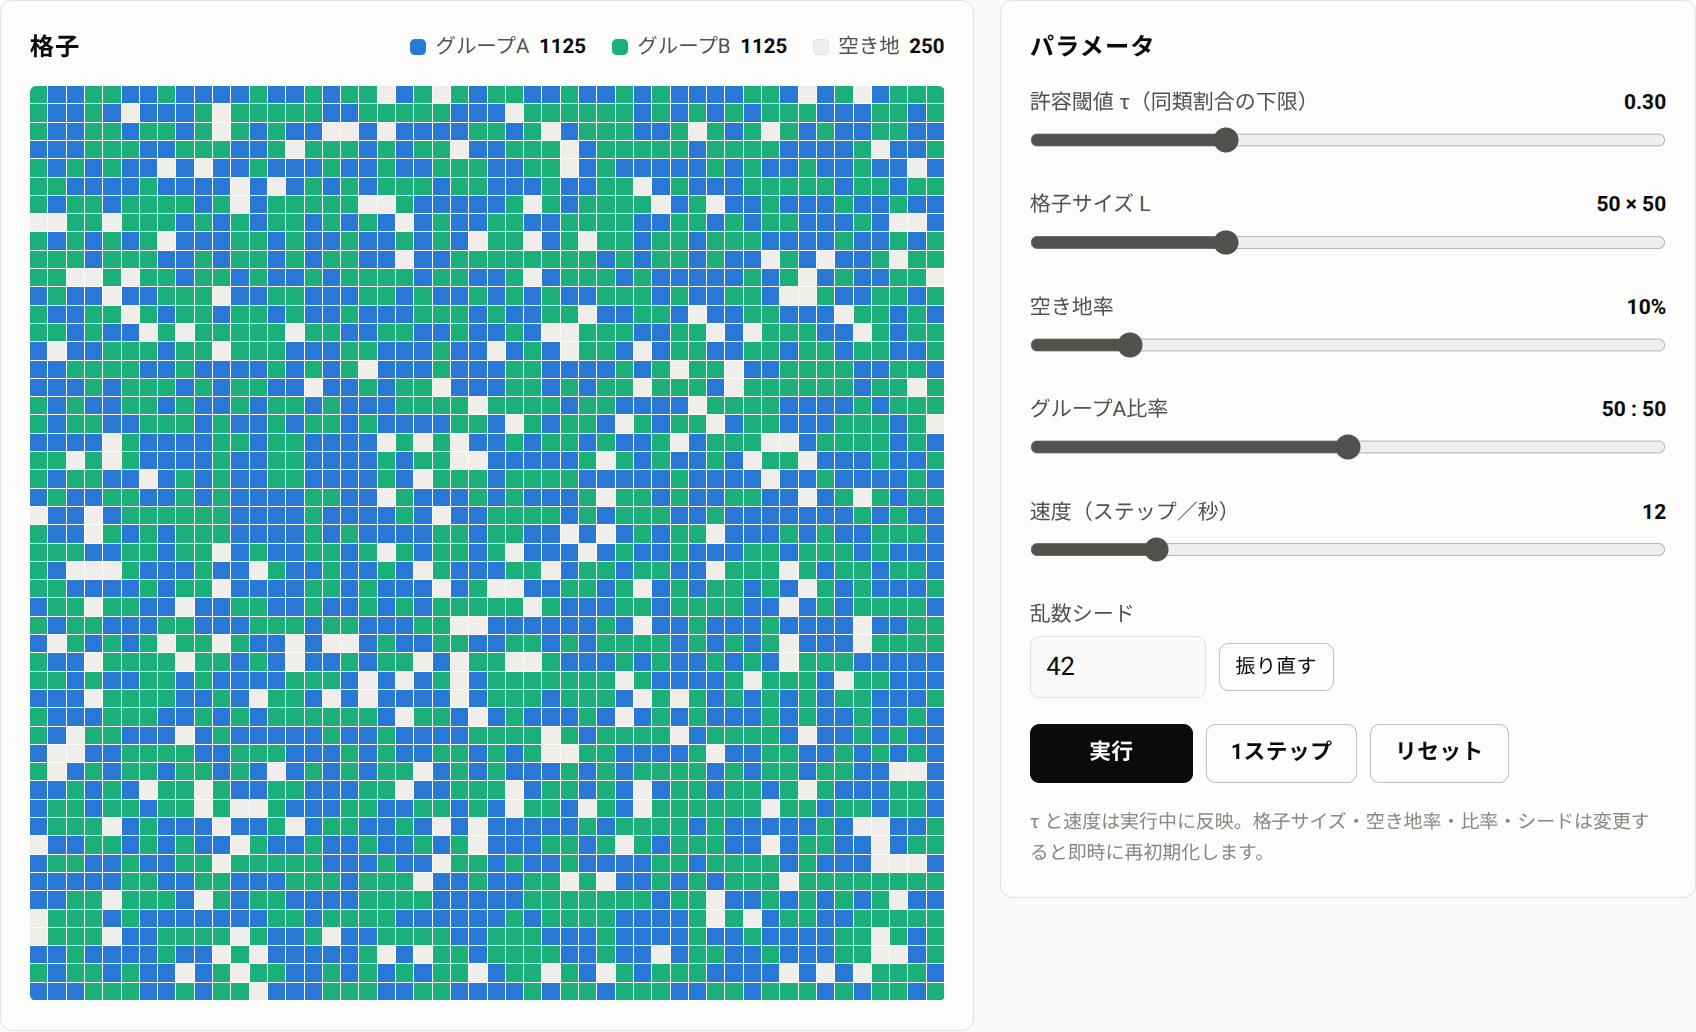
\includegraphics[width=\linewidth]{figures/schelling-initial.png}
\caption{シェリング分居モデルの初期画面（$L=50$，$v=0.10$，50:50，シード 42，ライトテーマ表示）．左：ランダム混住の格子（平均同類近傍率 49.4\%）と凡例（グループ別個体数）．右：パラメータパネルと実行制御．}
\label{fig:schelling-ui}
\end{figure}

\subsection{実装}

再現性の要は，シード付き乱数生成器 mulberry32 である（リスト\ref{lst:rng}）\footnote{Tommy Ettinger 作の 32 ビット状態の生成器（\url{https://gist.github.com/tommyettinger/46a874533244883189143505d203312c}）．JavaScript 標準の \texttt{Math.random()} にはシード指定機能がないため，シード付き乱数を 1 行数十文字で書ける手軽さから事実上の定番となっている．}．初期配置のシャッフルと移動先の選択がすべてこの生成器を通るため，同じシードと設定なら同じ軌道が完全に再現される．

\begin{lstlisting}[caption={シード付き乱数生成器 mulberry32},label={lst:rng}]
function mulberry32(seed){
  var a = seed >>> 0;
  return function(){
    a |= 0; a = (a + 0x6D2B79F5) | 0;
    var t = Math.imul(a ^ (a >>> 15), 1 | a);
    t = (t + Math.imul(t ^ (t >>> 7), 61 | t)) ^ t;
    return ((t ^ (t >>> 14)) >>> 0) / 4294967296;
  };
}
\end{lstlisting}

1 ステップ（スイープ：不満エージェント全体をひと巡り処理すること）の中核はリスト\ref{lst:sweep}のとおり．空き地リストに対する「選んだ空き地を移動元セルで置き換える」スワップ（入れ替え）操作により，空き地の一様抽選を $O(1)$（空き地の数が増えても処理時間が変わらない，の意の計算量記法）で維持している．格子は \texttt{Int8Array}，近傍はトーラス上のオフセットを事前計算した \texttt{Int32Array}（いずれも高速・省メモリの数値専用配列）で保持し，$L=120$（14{,}400 セル）でも毎秒 60 ステップの実行が可能である．

\begin{lstlisting}[caption={スイープ（1ステップ）の中核部},label={lst:sweep}]
// enumerate unsatisfied agents at sweep start, shuffle,
// then move each to a uniformly random vacant cell
var moves = 0;
for(var m = 0; m < unsatList.length; m++){
  if(vacant.length === 0) break;
  var from = unsatList[m];
  var vi = (rng() * vacant.length) | 0;
  var to = vacant[vi];
  vacant[vi] = from;   // vacated cell replaces the chosen vacancy
  grid[to] = grid[from]; grid[from] = 0;
  moves++;
}
\end{lstlisting}

\subsection{可視化設計とパレット検証}\label{sec:palette}

可視化は \texttt{dataviz} スキルの手順に従った．エンティティごとに固定順で色を割り当て（グループ A = 青，グループ B = アクア，平均同類近傍率 = 黄，満足率 = 緑；空き地はデータでないため無彩色），全系列を検証スクリプトにかけた．結果の要点：

\begin{itemize}
  \item 格子の 2 色（青・アクア）：CVD 分離 $\Delta E = 73.6$（ライト面）／$69.8$（ダーク面）で，目標値 12 を大きく上回り合格．
  \item チャートの 2 色（黄・緑）：ライト面で黄のコントラスト比 2.11（基準の 3:1 未満の警告）→ 救済条件として凡例への現在値常時表示・ツールチップ（マウスを重ねると現れる数値表示）・統計タイル（主要数値を大きく示すカード表示）を設置．ダーク面で $\Delta E = 10.3$（下限帯 8--12）→ 直接ラベルの併設により許容．
\end{itemize}

「警告は救済条件（可視ラベル等の第二の情報チャネル）とセットでのみ許容される」という規範が，機械判定によって強制される点が本手法の特長である．このほか，2 指標はいずれも割合（0--1）であるため単一の縦軸（0--100\%）を共有させ，二重軸を回避した．時系列チャートにはクロスヘア（照準線）付きツールチップを実装し，全履歴を CSV（comma-separated values）\footnote{カンマ区切りのテキスト形式．表計算ソフトや統計ソフトでそのまま読み込める．}としてクリップボードに出力するボタンを設けて外部解析への接続点とした．

\subsection{分析結果}\label{sec:analysis}

以下の数値は，アーティファクトと同一のアルゴリズム・同一の乱数生成器を Node.js で再現実行して得たものであり，アーティファクト上でも同じシードを入力すれば同じ軌道が観察できる\footnote{Node.js の併用は分析上の必然ではなく，バッチ実行の足場としての選択である．基準実行のような単一の実行は，アーティファクト単体で観察から CSV 出力まで完結する．一方，後述の許容閾値スイープは 8 水準 $\times$ 10 シードの計 80 回の実行と集計を要し，描画と同期した対話的実行を UI 操作で繰り返して手作業で集計するのは現実的でない．描画を切り離した Node.js では全 80 回の実行が数秒で完了し，結果をそのまま表\ref{tab:sweep}に整形できる．なお，両環境の結果が桁まで一致すること（図\ref{fig:schelling-live}）は，この再現実装の正しさの検証を兼ねている．}．

\paragraph{基準実行}
$L=50$，$v=0.10$，グループ比 50:50，$\tau=0.30$，シード 42 の基準実行では，初期配置の平均同類近傍率は $\bar{s}_0 = 0.494$（ランダム混住の理論値 0.5 と整合）で，初期満足率はすでに 82.7\%である．すなわち大多数のエージェントは初期状態に満足している．それにもかかわらず，わずか 14 ステップ（延べ 1{,}003 回の移動）で全員満足に収束し，最終的な平均同類近傍率は $\bar{s} = 0.741$ に達した（図\ref{fig:traj}）．「同類が 3 割いれば満足」という穏やかな個人選好が，74\%という強い集団的分居を生む—シェリングが示した創発\footnote{個々の主体の単純な行動の相互作用から，誰も意図しないマクロな秩序が生じること．}の核心が，そのまま再現されている．

この基準実行はアーティファクト上でもそのまま観察できる．図\ref{fig:schelling-conv}は収束時点の格子で，初期のランダム混住（図\ref{fig:schelling-ui}）から同色のクラスタが明瞭に形成され，パネル上部に収束バッジ（ステップ 14）が点灯している．収束後は「実行」「1 ステップ」が無効化され，パラメータを変えるまで系が静止したことが操作面からも分かる．図\ref{fig:schelling-live}は同時点の統計タイルと時系列チャートである．表示値（平均同類近傍率 74.1\%・満足率 100.0\%）は，Node.js による再現実行（図\ref{fig:traj}）と桁まで一致しており，ブラウザ上のライブ実行とオフライン再現が同一の軌道をたどることが画面上でも確認できる．

\begin{figure}[tbp]
\centering
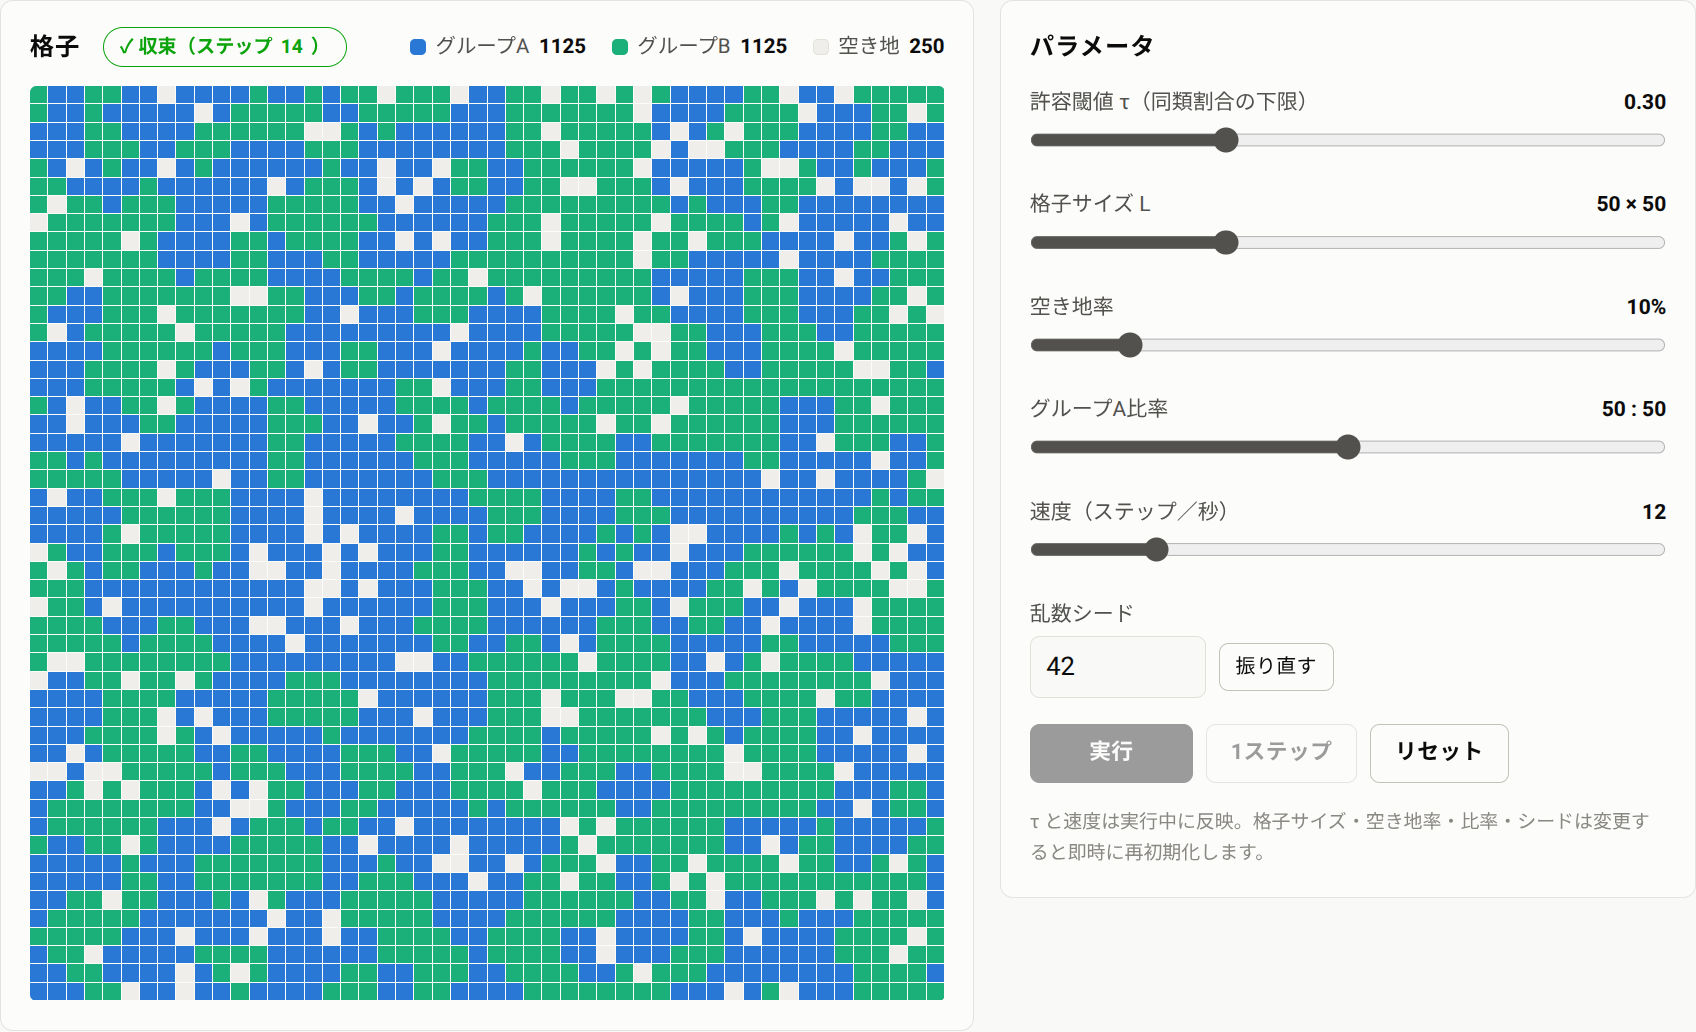
\includegraphics[width=\linewidth]{figures/schelling-converged.png}
\caption{収束後の格子（ステップ 14，$\tau=0.30$，シード 42）．同色クラスタが形成され，収束バッジが点灯する．収束により「実行」「1 ステップ」ボタンは無効化されている．}
\label{fig:schelling-conv}
\end{figure}

\begin{figure}[tbp]
\centering
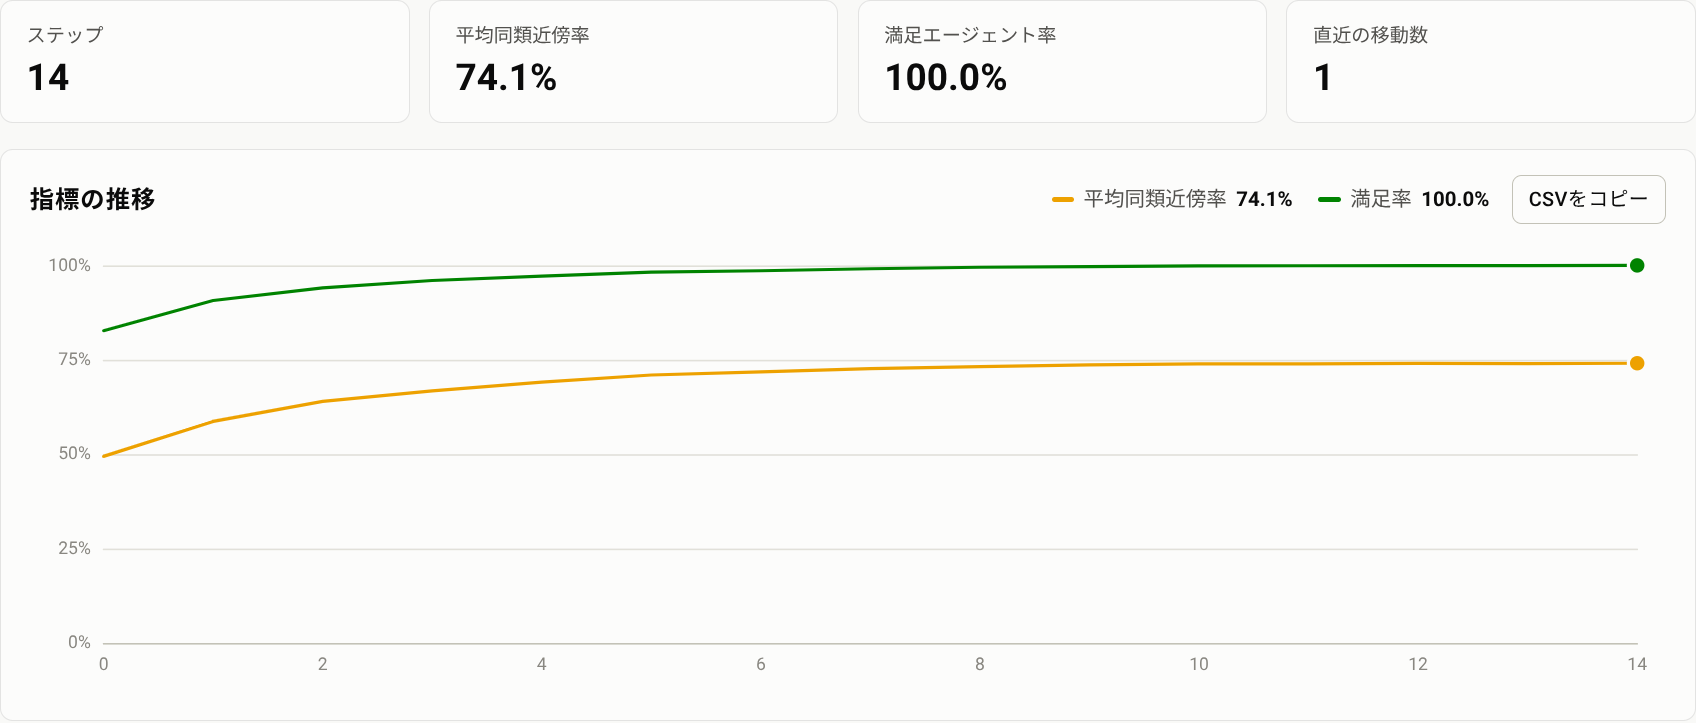
\includegraphics[width=\linewidth]{figures/schelling-chart.png}
\caption{収束時点の統計タイルと指標チャート．平均同類近傍率 74.1\%・満足率 100.0\%は再現実行（図\ref{fig:traj}）と一致する．凡例には現在値が常時表示され，ライトモードで 3:1 未満となる黄系列のコントラスト警告に対する救済チャネルを構成する（第\ref{sec:palette}節）．}
\label{fig:schelling-live}
\end{figure}

\begin{figure}[tbp]
\centering
\begin{tikzpicture}
\begin{axis}[
  width=0.85\linewidth, height=6.2cm,
  xlabel={ステップ}, ylabel={割合},
  xmin=0, xmax=14, ymin=0.4, ymax=1.02,
  ytick={0.4,0.5,0.6,0.7,0.8,0.9,1.0},
  yticklabel={\pgfmathprintnumber[fixed,precision=1]{\tick}},
  grid=major, grid style={black!12},
  axis line style={black!40},
  legend pos=south east, legend style={draw=black!25, font=\small},
  tick label style={font=\small}, label style={font=\small}
]
\addplot[segcol, thick, mark=*, mark size=1.6pt] coordinates {
  (0,0.4942) (1,0.5868) (2,0.6399) (3,0.6679) (4,0.6908) (5,0.7097)
  (6,0.7182) (7,0.7264) (8,0.7321) (9,0.7363) (10,0.7392) (12,0.7403) (14,0.7409)
};
\addlegendentry{平均同類近傍率 $\bar{s}$}
\addplot[satcol, thick, mark=square*, mark size=1.5pt] coordinates {
  (0,0.8271) (1,0.9071) (2,0.9404) (3,0.9600) (4,0.9716) (5,0.9822)
  (6,0.9858) (7,0.9911) (8,0.9951) (9,0.9969) (10,0.9987) (12,0.9996) (14,1.0000)
};
\addlegendentry{満足率}
\end{axis}
\end{tikzpicture}
\caption{基準実行の軌道（$L=50$，$v=0.10$，50:50，$\tau=0.30$，シード 42）．14 ステップで収束し，平均同類近傍率は 0.494 から 0.741 へ上昇する．}
\label{fig:traj}
\end{figure}

\paragraph{許容閾値のスイープ}
$\tau$ を変化させ，各 10 シード（1--10）・上限 3{,}000 ステップで実行した結果を表\ref{tab:sweep}と図\ref{fig:sweep}に示す．

\begin{table}[tbp]
\centering
\caption{許容閾値 $\tau$ のスイープ（$L=50$，$v=0.10$，50:50，シード 1--10，上限 3{,}000 ステップ）}
\label{tab:sweep}
\begin{tabular}{ccccc}
\toprule
$\tau$ & 最終 $\bar{s}$（平均） & 標準偏差 & 平均収束ステップ & 収束数 \\
\midrule
0.10 & 0.511 & 0.006 & 1.4 & 10/10 \\
0.20 & 0.576 & 0.014 & 6.4 & 10/10 \\
0.25 & 0.581 & 0.015 & 6.2 & 10/10 \\
0.30 & 0.750 & 0.011 & 12.6 & 10/10 \\
0.40 & 0.826 & 0.010 & 16.1 & 10/10 \\
0.50 & 0.867 & 0.006 & 17.4 & 10/10 \\
0.60 & 0.974 & 0.001 & 131.0 & 10/10 \\
0.70 & 0.995 & 0.001 & 207.6 & 10/10 \\
\bottomrule
\end{tabular}
\end{table}

\begin{figure}[tbp]
\centering
\begin{tikzpicture}
\begin{axis}[
  width=0.85\linewidth, height=6.2cm,
  xlabel={許容閾値 $\tau$}, ylabel={最終 $\bar{s}$（10 シード平均）},
  xmin=0.05, xmax=0.75, ymin=0.45, ymax=1.02,
  grid=major, grid style={black!12},
  axis line style={black!40},
  tick label style={font=\small}, label style={font=\small}
]
\addplot[segcol, thick, mark=*, mark size=2pt] coordinates {
  (0.10,0.5114) (0.20,0.5762) (0.25,0.5805) (0.30,0.7495)
  (0.40,0.8259) (0.50,0.8670) (0.60,0.9743) (0.70,0.9950)
};
\end{axis}
\end{tikzpicture}
\caption{許容閾値 $\tau$ と最終的な平均同類近傍率の関係．$\tau=0.25 \to 0.30$ で不連続に跳躍する．}
\label{fig:sweep}
\end{figure}

三つの特徴が読み取れる．第一に，$\tau$ と分居度の関係は単調だが強く非線形であり，特に $\tau = 0.25 \to 0.30$ で $\bar{s}$ が $0.58$ から $0.75$ へ不連続に跳躍する．これはムーア近傍の離散性による．占有近傍が 8 のとき，満足に必要な同類数は $\lceil 8\tau \rceil$（$8\tau$ 以上で最小の整数）であり，$\tau=0.25$ では 2 人，$\tau=0.30$ では 3 人と，実効閾値が整数単位で切り替わるためである．連続パラメータの背後にある離散構造が集計量に現れる好例であり，講義での議論素材に適する．

第二に，$\tau=0.10$ では $\bar{s} = 0.511$ と初期値からほとんど動かない．不満者が僅少のため 1--2 ステップで収束し，分居はほぼ生じない．創発的分居には「穏やかだがゼロではない」選好水準が必要であることがわかる．

第三に，$\tau \ge 0.60$ の高選好域では，最終分居度が 0.97 を超えて飽和する一方，収束までの平均ステップ数が 131（$\tau=0.6$），208（$\tau=0.7$）と一桁以上増大する．要求水準が高いほど「引っ越しの連鎖」が長く続き，ほぼ完全な棲み分け（少数の巨大クラスタ）に達してようやく停止する．なお空き地率 10\%の本設定では上限 3{,}000 ステップ内に全実行が収束したが，$\tau$ をさらに上げれば非収束（エージェントの引っ越しが永久に続く churning と呼ばれる状態）に転じることが知られている．

\subsection{再現性の担保}

以上の分析はすべて，(1) シード付き乱数による軌道の完全な決定性，(2) アーティファクトの CSV 出力（\texttt{step, mean\_like\_neighbor\_frac, satisfied\_frac, moves}），の二点によって，アーティファクト上でもオフライン解析でも同一に再現できる．この「ブラウザ内のデモが同時に再現可能な計算実験装置でもある」という性質は，教材と研究ツールの距離を縮めるものである．

\section{議論}\label{sec:discussion}

\subsection{教育・研究上の含意}

本稿の二事例が示すように，アーティファクトによるシミュレーション構築は (1) 配布物が URL 一つ，あるいは自己完結した HTML ファイル一つで済むこと，(2) 実行環境がブラウザのみであること，(3) シードによる再現性，という三点で教育利用に適する．講義では受講者が各自のデバイスでパラメータを操作でき，演習では CSV 出力を起点に統計解析へ接続できる．研究面では，モデルの挙動を共同研究者に伝える「動く補足資料」としての利用が現実的である．

配布方法は，所属機関の契約形態に応じて使い分けることになる．大学が Claude for Education（大学向けの組織契約プラン）\cite{anthropic-education}を導入している場合，アーティファクトの共有は組織内共有型（第\ref{sec:artifact}節）となるため，学生が大学アカウントでログインする前提で「URL 一つの学内配布」が成立する．受講者全員が同じ組織に属する講義利用には，この形態はむしろ好適である．一方，組織の壁を越える共有手段はないため，学外の読者・査読者・他大学の受講者への配布には，自己完結した HTML ファイルの直接配布か，GitHub Pages による公開（第\ref{sec:ghpages}節）を用いる．

\subsection{限界と対処}

第\ref{sec:constraints}節の制約から，大規模計算（数十万エージェント超，長時間の実行，広範なパラメータスイープ）には向かない．この場合は，計算を Python の ABM ライブラリ Mesa や科学計算向け言語 Julia などで別途実行し，軌道データを埋め込んだ再生ビューアとしてアーティファクトを設計する二段構成が有効である．スイープ結果のヒートマップ（値の大小を色の濃淡で示す図）から特定の実行の再生に遷移する構成も同じ枠組みで実現できる．また，アーティファクトは既定で非公開であり，Web 上での共有は同一組織内に限られる点（組織外への配布には，HTML ファイルの直接配布のほか，次項で述べる GitHub Pages による公開が使える），および外部データの動的取得ができない点には留意されたい．

\subsection{代替配布手段：GitHub Pages による公開}\label{sec:ghpages}

アーティファクトの Web 共有は前述のとおり組織内（個人プランでは本人のみ）に限られるが，講義や学会発表では「URL を配れば誰でも開ける」形の公開が欲しい場面が多い．この目的には GitHub Pages が適する．GitHub Pages は，ソースコード共有サービス GitHub が無料で提供する静的サイトホスティング（HTML 等のファイルをそのまま Web サイトとして配信するサービス）である\cite{github-pages}．アーティファクトとして作られた HTML は，第\ref{sec:constraints}節の制約ゆえに完全に自己完結している（外部のライブラリやフォントを一切参照しない）ため，静的ホスティングとの相性が極めて良い．ファイルを 1 つ置くだけで，そのまま動く．

手順は次のとおりである．

\begin{enumerate}
  \item GitHub にアカウントを作成し，リポジトリ（ファイル置き場）を新規作成する（例：\texttt{my-simulations}）．
  \item アーティファクトの HTML ファイルをリポジトリに追加する（例：\texttt{schelling.html}）．Claude Code を使っていれば，「この HTML を GitHub に追加してプッシュして」と依頼するだけで，コミット（変更の記録）とプッシュ（GitHub への送信）まで代行される．
  \item リポジトリの Settings → Pages で，公開するブランチ（通常 \texttt{main}）とフォルダ（\texttt{/}）を指定する．
  \item 数分以内に \texttt{https://ユーザー名.github.io/リポジトリ名/schelling.html} で公開される．以後，ファイルを更新してプッシュするたびに，同じ URL の内容が更新される．
\end{enumerate}

この方式の利点は，(1) 無料で恒久的な公開 URL が得られ，閲覧に GitHub や \texttt{claude.ai} のアカウントを要しないこと，(2) Git による履歴管理が残り「どの版を配布したか」を後から特定できること，(3) アーティファクトと同じく「再プッシュで同一 URL の内容を更新する」運用ができること，である．留意点は二つある．第一に，公開リポジトリではソースコード（HTML の中身）もそのまま公開される．第二に，GitHub Pages 上の複製は \texttt{claude.ai} 上のアーティファクトとは独立であり，アーティファクト側を更新しても自動では反映されない（更新のたびに再プッシュが必要である）．

\section{おわりに}

本稿では，Claude Code のアーティファクト機能によるシミュレーション構築を，機能解説と二つの実例（連続時間の遊戯的シミュレータ，標準仕様のシェリング分居モデル）を通じて示した．とりわけ後者では，対話による仕様確定から，検証スクリプトに裏付けられた可視化設計，シード付き乱数による再現可能な分析までの全過程が，単一の HTML ファイルと URL に収まることを確認した．ABM の教育・研究における「触れるモデル」の敷居は，確実に下がっている．

\appendix

\section{公開アーティファクト一覧}

\begin{itemize}
  \item 炭火職人（うなぎ蒲焼きシミュレータ）\\
    \url{https://claude.ai/code/artifact/100b5bc4-c60e-42cd-9e19-f9277dbb6685}
  \item シェリング分居モデル（ライブ ABM）\\
    \url{https://claude.ai/code/artifact/9ac47541-7715-48f8-9513-39ef5e4c9772}
\end{itemize}

いずれも既定で非公開である（共有できる範囲については第\ref{sec:artifact}節を参照）．

\begin{thebibliography}{9}
\bibitem{anthropic-claudecode}
Anthropic, ``Claude Code Documentation,''
\url{https://code.claude.com/docs/}（2026年7月13日閲覧）．
\bibitem{anthropic-artifacts}
Anthropic, ``Share Session Output as Artifacts,''
\textit{Claude Code Documentation},
\url{https://code.claude.com/docs/en/artifacts}（2026年7月13日閲覧）．
\bibitem{anthropic-publish}
Anthropic, ``Publish and Share Artifacts,''
\textit{Claude Help Center},
\url{https://support.claude.com/en/articles/9547008-publish-and-share-artifacts}（2026年7月13日閲覧）．
\bibitem{anthropic-education}
Anthropic, ``Introducing Claude for Education,''
\url{https://www.anthropic.com/news/introducing-claude-for-education}（2026年7月13日閲覧）．
\bibitem{github-pages}
GitHub, ``GitHub Pages Documentation,''
\url{https://docs.github.com/en/pages}（2026年7月13日閲覧）．
\bibitem{schelling1971}
Schelling, T.~C. (1971) ``Dynamic Models of Segregation,''
\textit{Journal of Mathematical Sociology}, 1(2), 143--186.
\end{thebibliography}

\end{document}
